\documentclass[12pt]{article}

\usepackage{geometry}
\usepackage[T1]{fontenc}
\usepackage[utf8]{inputenc}
\usepackage[francais]{babel}

\usepackage{graphicx}
\usepackage{lmodern}

\geometry{margin=2cm}

\newcommand {\ST}{Sven Taton}
\newcommand {\QL}{Qiwen Lu}
\newcommand {\LL}{Louis Le Clec'h}
\newcommand {\DB}{David Bitonneau}
\newcommand {\AH}{Arthur Havlicek}
\newcommand {\BR}{Benoit Ruelle}
\newcommand {\LH}{Ludovic Hofer}

\newcommand{\HRule}{\rule{\linewidth}{0.5mm}}


\title{}
\author{\ST\\\QL\\\LL\\\DB\\\AH\\\BR\\\LH}

\begin{document}

\begin{center}
	\begin{tabular*}{\textwidth}{l @{\extracolsep{\fill}} r}

      %\hline
		
\includegraphics [width=40mm]{ENSEIRB-MATMECA.ps} & 
\includegraphics
		[width=40mm]{logo-LaBRI-couleur.ps}\\
      %\hline

    \end{tabular*}
    
\vspace{\stretch{1}}
      
    \textsc{\Huge Document de spécification des besoins}\\[0.5cm]
	\rule{0.4\textwidth}{1pt}
           
\vspace{\stretch{1}}
           
                  %{\huge \bfseries \reporttitle}\\[0.4cm]
                  %\HRule \\[1.5cm]
                  
                  \begin{center}
                    
                    \begin{flushleft} 
                      \large
                      \emph{Auteur :}\\
                      \begin{itemize}
                        \item Arthur Havlicek
						\item Benoît Ruelle
                        \item David Bitonneau
                        \item Louis Le Clec'h
                        \item Ludovic Hofer
                        \item Qiwen Lu
                        \item Sven Taton
                      \end{itemize}
                    \end{flushleft}
                    
                    
                    \begin{flushright} 
                      \large
                      \emph{Responsables :} \\
					  {\small pédagogique} - M.~Renault \\
						  {\small client} - M.~Le Borgne\\
                    \end{flushright}
                  \end{center}
                  
                  
                  %\vfill                  
\vspace{\stretch{1}}
                  
{\large Deuxième année, filière informatique}

~

{\large 16 octobre 2012 - 29 mars 2013}\\
                  
\end{center}
\thispagestyle{empty}
\pagebreak

%%%%%%%%%%%%%%%%%%%%%%%%%%%%%%%%%%%%%%%%%%%%%%%%%%%%%%%%%%%%%%%%%%%%%%%%%%%%
%\begin{center}
%	{\Huge{Un bot pour NetHack \\ \vspace{2cm} Document de spécification des b%esoins}}
%\end{center}

%\vspace{2cm}

%\noindent {\large Auteurs : Sven Taton, Qiwen Lu, Louis Le Clec'h, David Bitonneau, Arthur Havlicek, Benoît Ruelle, Ludovic Hofer}


%\vspace{4.2cm}

%\noindent{\large{Client : Yvan Le Borgne}}\\
%\noindent{\large{Responsable pédagogique : David Renault}}
%\pagebreak
%%%%%%%%%%%%%%%%%%%%%%%%%%%%%%%%%%%%%%%%%%%%%%%%%%%%%%%%%%%%%%%%%%%%%%%%%%%%%
\section{Introduction}

Nethack est un jeu vidéo de type rogue-like écrit en C sous licence libre. Le joueur incarne un aventurier chargé par son dieu/sa déesse de récupérer une amulette dans un donjon peuplé de monstres et de trésors. Le jeu se présente sous la forme d'une grille composées de salles, de couloirs les reliant et se joue au tour par tour. Plusieurs interfaces sont proposées : de la représentation en texte en utilisant des codes d'echapement du terminal à l'interface graphique en Qt ou GTK.

L'objectif du projet est d'adapter le jeu pour la résolution de problèmes
isolés de NetHack par des bots. Il s'agit donc dans un premier temps de produire une base pour la
création de bots en fournissant un moyen pour les bots d'interagir avec le jeu
et permettant la génération de statistiques. Dans un second temps, définir des sous-problèmes du jeu et de créer des bots pouvant évoluer dans les modes de jeux correspondant à ces problèmes, et ainsi permettre la validation de modèle théorique par leur application sur le jeu.


\section{Modèle conceptuel}

Il est demandé qu'une version validant le modèle soit fonctionnel très rapidement, afin de satisfaire cet exigence sans pour autant laisser de côtés les qualités attendues d'un logiciel, deux versions différentes seront présentées : un prototype et une version plus intégrée au noyau.

\subsection{Le prototype}
Afin que le prototype ne nécessite pas trop de temps de développement, il sera simplifié par rapport au contenu final du projet. Le fonctionnement de l'interface sera inspiré de celui de TAEB, elle sera écrite en Perl et assurera deux rôles :
\begin{itemize}
\item La traduction de la sortie sur un terminal du jeu vers un protocole
simple compris par les bots.
\item Traduction et transmission des actions choisies par le bot au noyau.
\end{itemize}
Le prototype permettra en outre de faire jouer les bots sur des versions
originales du jeu n'ayant subit aucune modification.

\begin{center}
  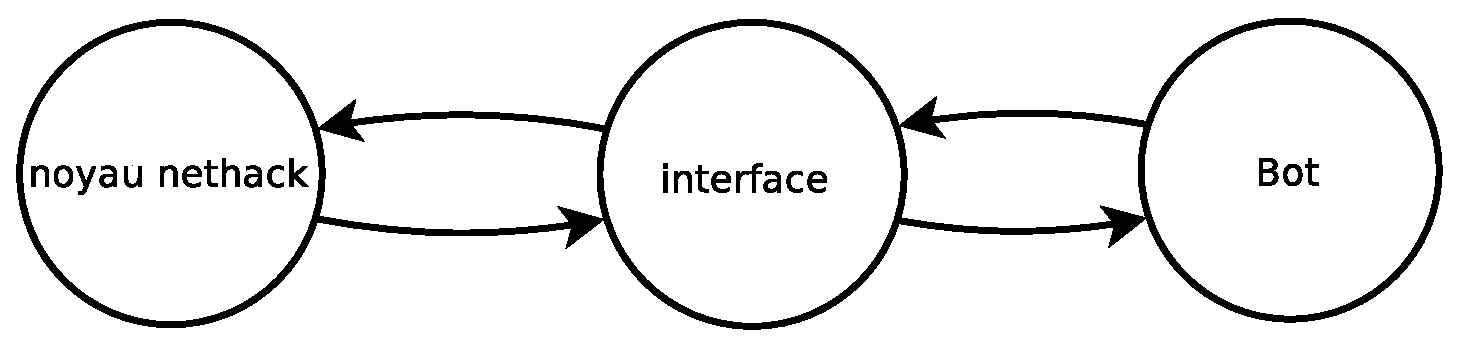
\includegraphics[width=180mm]{diagrammes/proto_archi.eps}
\end{center}

\subsection{L'architecture du logiciel}
\begin{center}
  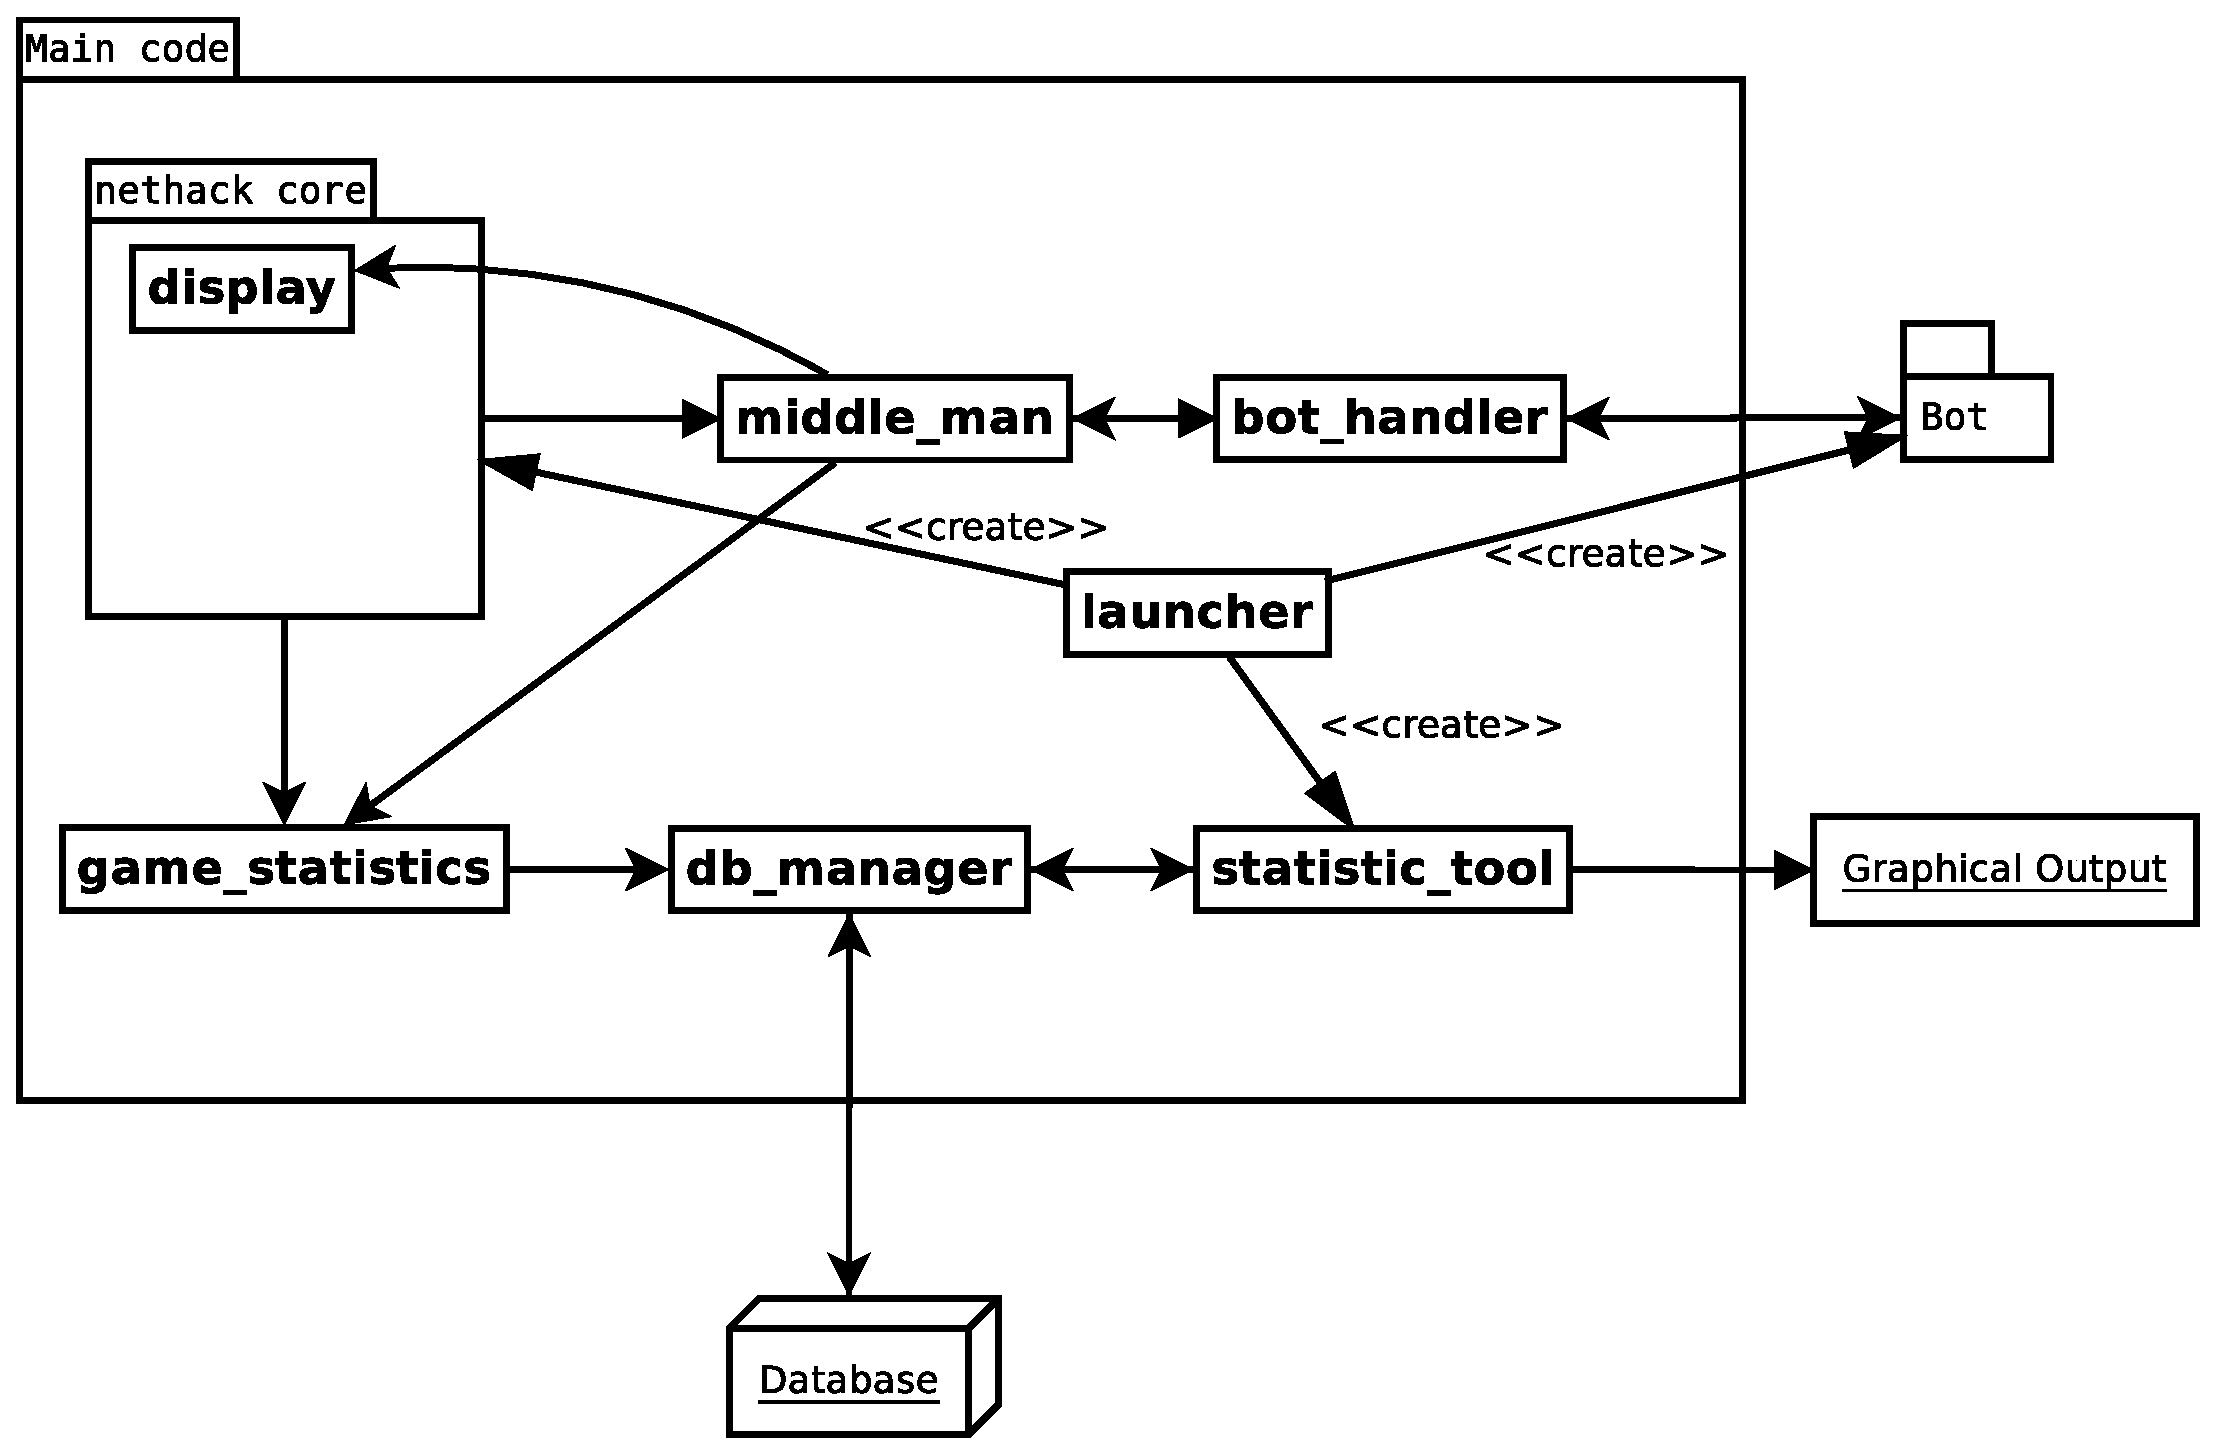
\includegraphics[width=180mm]{diagrammes/new_archi.eps}
\end{center}

\subsubsection*{Main code}
Ce code source sera écrit en C et viendra compléter nethack.
\subsubsection*{Game Launcher}
Le lanceur permettra de créer un processus pour nethack puis un processus pour le bot. Il permettra aussi de choisir entre différentes options propre à nos ajouts concernant nethack.
\subsubsection*{Middle man}
Cette partie viendra remplacer l'interface usuelle afin de capter directement la sortie de nethack. Les chaînes de caractères transmises aux différents affichages seront donc interprétées afin de reconstruire une représentation avant d'être envoyée au module d'affichage initialement prévu.
La représentation structurée sera retransmise au bot handler. En fin de partie, un appel à game\_statistics permettra de remplir la base de données.
\subsubsection*{Bot handler}
Ce module se sert d'informations structurées pour envoyer des messages faciles
à parser aux bots. Il traduira aussi les actions choisies par le bot en
actions NetHack et devra assurer le retour à la boucle principale du jeu après
chaque commande transmise au noyau pour maintenir la synchronisation entre les
bots et NetHack.
\subsubsection*{Game statistics}
Ce module permettra d'accéder aux données qui serviront de point de comparaison des bios,
\subsubsection*{Database manager}
Ce module permettra d'ajouter le résultat de parties à la base de données, mais il permettra aussi d'exécuter des requêtes sql sur les tables.
\subsubsection*{statistic tool}
Cet outil servira à analyser les performances de nos divers bots et à décider lequel est le plus efficace.


\section{Besoins fonctionnels}

\subsection{Communication avec NetHack}

Le projet doit fournir une interface permettant à des bots de jouer à NetHack. Elle consiste en un module ajouté au jeu assurant la liaison entre le jeu et les différentes parties du projet (bots, base de données, outil de statistiques).

Cette interface doit arbitrer les échanges entre les bots et le noyau. Par exemple, elle doit permettre de prouver que les bots ne puissent pas tricher et gérer gracieusement les erreurs provenant des différents éléments intervenants dans la simulation d'une partie.

\subsection{Création de `modes' de jeu}

Le projet devra établir au moins un mode de jeu correspondant à une modification du noyau de NetHack, une liste d'ordres permis aux bots, un ensemble de paramètres introduits à l'exécution et d'informations collectées sur une partie. L'ensemble formant un environnent pour la résolution d'un problème isolé du jeu.

\subsection{Collecte de statistiques}

Le projet devra alimenter une base de données à partir de parties jouées par des bots et des statistiques recueillies. Elles seront utilisées dans un système d'analyse de statistiques. Celles-ci seront prélevées à divers endroits : auprès des bots et auprès du noyau du jeu et rassemblées dans une base de données permettant d'effecteur des calculs statistiques ultérieurement.

\subsection{Analyse et présentation des statistiques}

Un outil d'analyse de statistiques devra être livré. Il permettra, entre autres, de comparer les performances des bots en termes de taux de réussite et de rapidité de différents algorithmes. Plus généralement, une mesure de pertinence telle que l'écart-type devra être affichée ou intégrée.

Il est souhaitable qu'il intègre un outil générant des graphiques pour une interprétation plus aisée.

\subsection{Outil de replay}

Pour la maintenance des bots, il est souhaitable de disposer d'un outil permettant de rejouer une partie ; soit passivement pour identifier une erreur dans l'algorithme d'un bot ; soit activement pour permettre de tester une correction dans l'algorithme d'un bot dans une situation où il avait échoué.

\section{Démarches et études}

Le projet devra se baser sur l'étude de problèmes spécifiques liés au jeu Nethack. L'objectif attendu par le client n'est pas de fournir des bots étant capable de jouer à Nethack, mais au contraire de mettre en place un cadre d'étude de sous-problèmes pouvant être révélés par l'étude du jeu.

Chaque sous-problème sera lié à un ``mode'' de jeu, c'est-à-dire un environnement - défini de façon formelle - dans lequel pourront évoluer des bots spécifiques. Cet environnement est défini par : 
\begin{itemize}
	\item un jeu d'actions autorisées pour les bots (ce jeu d'action est un sous-ensemble du jeu d'action de base) 
	\item la suppression de certaines contraintes telles que la faim, les pièges, etc. 
	\item un sous-ensemble de statistiques prélevée 
	\item un ensemble de paramètre servant à l'évaluation 
	\item des conditions de fin de jeu.
\end{itemize}

Les sous-problèmes suivant pourront faire l'objet d'une étude formelle : 
\begin{itemize}
	\item Exploration d'un niveau.
	\item Recherche de portes secrètes.
	\item Combat.
	\item \ldots
\end{itemize}

Chaque problème fera l'objet d'une approche algorithmique et probabiliste.

\subsection{Exemples d'études à réaliser}

\paragraph{Exploration d'un niveau :}

Ce problème correspond au problèmes de recherche de la sortie d'un labyrinthe.

Différents points peuvent être étudiés : 
\begin{itemize}
	\item Comment sortir le plus rapidement d'un niveau ? 
	\item Comment sortir du niveau en ayant exploré le plus de cases possibles ? 
	\item etc.
\end{itemize}


\paragraph{Recherche de portes secrètes :}

Dans le jeu original, une action permet d'effectuer des recherches dans l'environnement du personnage. Cette recherche peut entrainer la découverte de portes secrètes ou de passages secrets. Plusieurs études liées à cette particularité du jeu peuvent être effectuées : 
\begin{itemize}
	\item Avec limite de temps : 
	\begin{itemize}
		\item Comment trouver le plus de portes cachées, le plus vite possible ? 
		\item Comment trouver le plus de portes cachées, dans la limite de temps donnée ? 
		\item etc. 
	\end{itemize}
	\item Sans limite de temps : 
	\begin{itemize}
		\item Comment mettre le moins de temps possible pour trouver toutes les portes ? 
		\item etc.
	\end{itemize}
\end{itemize}

Le mode de jeu correspondant à la recherche des portes secrètes est défini selon les contraintes suivantes : 
\begin{itemize}
	\item Les actions autorisées par le personnage sont limitées aux déplacements, à l'action de recherche, à l'ouverture de portes, au changement de niveau. 
	\item Les contraintes suivantes sont supprimées : 
	\begin{itemize}
		\item la faim, 
		\item les pièges, 
		\item les monstres, 
		\item les objets. 
	\end{itemize}
	\item Les informations suivantes sont prélevées sur le noyau :
	\begin{itemize}
		\item nombre total de portes secrètes, 
		\item nombre de portes secrètes trouvées, 
		\item nombre de tours total 
	\end{itemize}
	\item La proportion des portes secrètes trouvées et le temps mis pour trouver ces portes seront évalués. 
	\item La fin du jeu aura lieu après une limite de temps donnée ou une fois que toutes les portes secrètes auront été trouvées.
\end{itemize}


\section{Besoins non fonctionnels}

Nous avons identifié les spécifications suivantes en terme de contraintes logicielles non fonctionnelles.

\subsection{Choix des sous-problèmes étudiés}

\begin{itemize}
	\item Les bots sont spécialisés dans la résolution d'un problème précis.  L'objectif n'est pas de créer un programme sachant jouer à NetHack dans sa version originale.
	\item Les sous-problèmes étudiés doivent être suffisamment vastes pour envisager plusieurs approches possibles.
\end{itemize}

\subsection{Modifications noyau}

\begin{itemize}
	\item Le code source principal doit être réalisé en langage C, en réutilisant au maximum les fonctionnalités déjà existantes dans NetHack. Ceci ne concerne pas les bots externes ni de potentiels scripts annexes comme un outil d'installation automatique.
	\item Les modifications devront être minimales et justifiées. Des modifications locales d'un nombre de lignes limités sont attendues sous la forme d'un fichier diff. Il sera nécessaire de pouvoir extraire ces modifications afin de permettre leur réapplication sur une version originale du jeu.  
	\item Les modifications doivent répondre à un besoin d'exécution et ne doivent pas permettre aux bots de tricher.
	\item L'ensemble logiciel doit pouvoir être installé facilement ; si des dépendances extérieures ont été nécessaires, elles doivent être listées et leur installation documentée.
\end{itemize}

\subsection{Interface et création de bots}

\begin{itemize}
\item L'interface doit permettre d'introduire de nouveaux bots aisément. Pour cela, le protocole de communication entre le bot et l'interface doit être spécifié. Des ``starter packs'' dans différents langages devront être fournis pour illustrer la démarche de création d'un bot.
\item L'outil de replay qu'elle proposera permettra de corriger le comportement des bots en fournissant un moyen de rejouer une partie pour identifier des erreurs ou valider les modifications apportées aux bots.
\item L'interface doit permettre de simuler de façon autonome un grand nombre de parties.
\item La stratégie employée par les bots doit être explicite. Leur fonctionnement doit soit pouvoir être déduit de leur code, soit documenté par ailleurs.
\end{itemize}

\subsection{Interprétation des statistiques et validation des stratégies}

\begin{itemize}
\item Le déroulement de parties doit fournir des statistiques, dans un format lisible et standard.
\item La production statistique doit pouvoir permettre de valider ou d'infirmer la pertinence de choix stratégiques des bots.
\item La différence de performance entre les bots doit pouvoir être expliquée à l'aide de raisonnements ou d'exemples.
\end{itemize}

\section{Sous-ensemble et priorités d'implémentation}

\begin{itemize}
\item Étudier le code source de NetHack et identifier les mécanismes de créations d'objets, de monstres, etc., afin d'évaluer la difficulté de création des modes.
\item Fournir un moyen de communication entre les bots, le jeu et un système de collecte de données sur les parties jouées.
\item Fournir une première version (éventuellement instable) présentant l'ensemble des fonctionnalités.
\item Produire des statistiques sur les données collectées.
\item Mettre en place au moins deux starter packages dont un en python
\item Développer la fiabilité du logiciel et fournir des versions améliorées des bots.
\item Être capable d'avoir un certain contrôle sur la génération de niveaux adaptés aux problèmes à résoudre.
\item Le développement d'autres modes et d'autres bots se fera pendant le temps restant.
\end{itemize}

\subsection{Organisation interne du travail}

La répartition du travail est faîte à l'aide du logiciel planner. Celui-ci
permet de modeler un diagramme de gantt et d'attribuer diverses ressources aux
tâches. Cette représentation permet de faire des attributions efficaces et
d'éviter un maximum que certaines tâches ralentissent les autres.\\

Comme le développement peut-être séparé en plusieurs parties différentes, nous
avons décidé de commencer par établir les interfaces de celles-ci afin que
chacun soit au clair sur ce qu'il doit développer et que les malentendus soient
évités autant que possible. Les fonctionnalités ne seront réellement développées
qu'une fois que les interfaces auront été clarifiées.\\

Des tests de recettes seront établis entre deux parties entretenant un contact
afin d'assurer que chacune remplisse bien le rôle que l'autre attend d'elle.\\

Une phase de test général précédera le développement des bots afin d'assurer la
résolution des derniers bugs.\\

Ce type de prévision permet par exemple de planifier qu'à la fin du projet, le
rapport commencera a être rédiger pendant que certains produiront et analyseront
des statistiques.\\

Le planning prévu sera joint à la fin du document.


\section{Information de maintenance}

\begin{itemize}
\item De nouveaux modes pourront être ajoutés plus tard dans la vie du logiciel, il convient donc de faire attention à rester libre à l'ajout de modes et de faciliter la création de ceux-ci.
\item De nouveaux bots dans d'autres langages sont susceptibles d'être développés, écrire un starter package doit donc rester simple.
\end{itemize}

\section{Glossaire}

\begin{itemize}
	\item Starter package : Bot volontairement simpliste pouvant servir de base à la création d'un bot sans avoir à réimplémenter les entrées/sorties avec l'interface.
	\item Mode : Configuration spécifique du jeu adaptée à un problème précis. Comprend :
  	\begin{itemize}
		\item Un ensemble de modifications du noyau
		\item Un jeu d'actions possibles avec certaines règles
		\item Un ensemble de paramètre servant à l'évaluation
		\item Des conditions de fin de jeu
  	\end{itemize}
	\item Rogue-like : jeu inspiré du jeu vidéo ``Rogue''. Le joueur incarne un aventurier explorant des souterrains dans lesquels il affronte des monstres tout en se frayant un chemin vers les niveaux inférieurs.
	\item Bot : programme informatique automatisant des actions dans un jeu ou simulant un joueur humain
\end{itemize}

\end{document}

%vim:tw=0
